\section{Experiments and Results}
\label{sec:experiments}

We organize 421 experiments (180 ML + 241 LLM) into four cross-domain findings. DTI uses a single seed; CT and PPI use 3 seeds (we report mean $\pm$ std). Full per-run tables appear in Appendices~B--C.

\subsection{Do Curated Negatives Differ from Controls?}
\label{sec:exp-inflation}

We train identical models on NegBioDB negatives versus uniform random and degree-matched control negatives, holding all other variables constant (Table~\ref{tab:ml_results}).

\textbf{DTI.} Degree-matched negatives inflate LogAUC by +0.112 on average across all three models (e.g., GraphDTA: 0.843 $\to$ 0.967). This confirms that assumed-negative benchmarks systematically overestimate model performance. Uniform random controls show negligible average inflation ($<$+0.01 LogAUC), indicating that degree matching specifically creates an especially easy discrimination task.

\textbf{CT.} The pattern reverses in direction: NegBioDB negatives (clinical failures) are trivially separable from CTO successes (AUROC~=~1.0), while control negatives are harder. Degree-matched controls reduce AUROC by 0.16--0.24 across models (e.g., GNN: 1.0 $\to$ 0.76). This is expected---genuine clinical failures carry rich pharmacological features absent from random drug--condition pairs.

\textbf{PPI.} The effect is \emph{model-dependent}---a novel finding. Sequence-based models (SiameseCNN, PIPR) show +0.03--0.05 LogAUC inflation with control negatives, consistent with DTI. However, MLPFeatures shows \emph{reversed} inflation: NegBioDB negatives are harder than controls ($-$0.03 to $-$0.11 LogAUC), because hand-crafted features (protein degree, subcellular localization) capture the same structural signal that curated negatives encode.

\textbf{Cross-domain insight.} Curated negatives carry systematically different signal than controls in all three domains. The \emph{direction} of inflation depends on whether the model architecture captures the same features that distinguish curated from random negatives.

\begin{table}[t]
\centering
\caption{ML results summary: best model per domain across key splits and negative source inflation. Cold-X/Y denote the domain-specific cold entity splits (drug/target for DTI, drug/condition for CT, protein/both for PPI). $\Delta$ reports the change in primary metric when switching from NegBioDB to degree-matched negatives.}
\label{tab:ml_results}
\small
\begin{tabular}{@{}llccccl@{}}
\toprule
\textbf{Domain} & \textbf{Model} & \textbf{Random} & \textbf{Cold-X} & \textbf{Cold-Y} & \textbf{DDB} & \textbf{Neg.\ Inflation} \\
\midrule
DTI & GraphDTA & .997 & .997 & .863 & .997 & +0.124 LogAUC \\
DTI & DrugBAN  & .997 & .997 & .760 & .997 & +0.125 LogAUC \\
\midrule
CT-M1 & XGBoost & 1.00 & 1.00 & 1.00 & --- & $-$0.16 AUROC \\
CT-M2 & XGBoost & .51{\scriptsize\,mF1} & .41 & .34 & --- & --- \\
\midrule
PPI\,(seq) & PIPR & .964 & .859 & \textbf{.409} & .964 & +0.03--0.05 LogAUC \\
PPI\,(feat) & MLPFeat & .962 & .931 & \textbf{.950} & .961 & \textbf{$-$0.03 to $-$0.11 LogAUC} \\
\bottomrule
\end{tabular}
\end{table}


\subsection{Does Cold Splitting Expose Generalization Failures?}
\label{sec:exp-cold}

Cold splits remove all instances of a specific entity from the training set, testing whether models generalize to unseen drugs, targets, proteins, or conditions (Figure~\ref{fig:heatmap}).

\textbf{DTI.} Cold-target splitting is catastrophic: LogAUC collapses from 0.83 to 0.15--0.33 across all three models, while AUROC misleadingly remains 0.76--0.89. DrugBAN suffers most severely (LogAUC~=~0.151, AUROC~=~0.760). Cold-compound splitting has minimal effect, indicating models memorize target-specific patterns.

\textbf{CT.} M1 binary classification remains trivially solvable even under cold splits (AUROC~=~1.0 for cold\_drug and cold\_condition). However, M2 7-way category prediction reveals severe failures: scaffold and temporal splits collapse macro-F1 to 0.19 across all models, approaching the random baseline of $1/7 \approx 0.14$.

\textbf{PPI.} Cold-both splitting (unseen proteins on both sides, via METIS partitioning) produces a model-dependent catastrophe. PIPR drops to AUROC~=~0.409---\emph{below random}---while MLPFeatures remains robust at 0.950. This 0.54 AUROC gap between sequence-based and feature-based architectures is the largest we observe. SiameseCNN falls in between (0.585).

\textbf{Cross-domain pattern.} Cold-split catastrophe is \emph{universal} across domains but \emph{model-dependent} within each domain. Sequence-based and attention models memorize training entities; feature-based models generalize. Notably, DDB $\approx$ random in all three domains, suggesting degree-balanced splitting does not add meaningful difficulty beyond random assignment.

\begin{figure}[t]
\centering
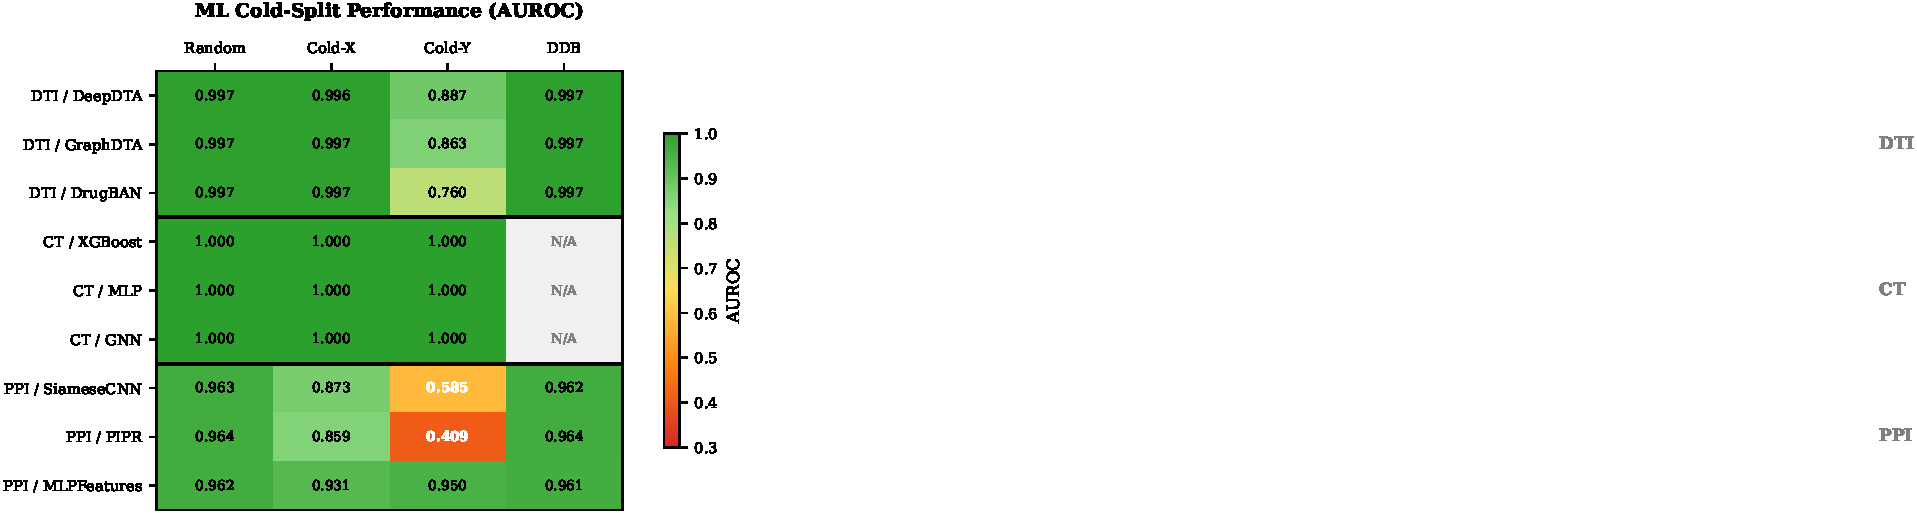
\includegraphics[width=0.65\textwidth]{figures/fig2_ml_heatmap.pdf}
\caption{ML cold-split performance across domains (AUROC). Red cells indicate catastrophic failure ($<0.7$). CT M1 is trivially separable across all splits; cold-both PPI reveals a 0.54 gap between sequence (PIPR: 0.409) and feature-based (MLPFeatures: 0.950) architectures. N/A: split not applicable.}
\label{fig:heatmap}
\end{figure}


\subsection{Can LLMs Reason About Negative Biological Evidence?}
\label{sec:exp-llm}

We evaluate five LLMs across four evaluation levels in each domain (Table~\ref{tab:llm_results}).

\textbf{L1 (Multiple Choice).} Performance varies dramatically by domain. PPI is trivially solvable: all models achieve $\geq$0.999 accuracy with 3-shot prompting (evidence text makes category self-evident). CT is the hardest domain: the best model (Gemini) reaches only 0.667 accuracy on 5-way classification, well below the 0.80+ levels seen in DTI and PPI. DTI falls between (0.65--1.0 with 3-shot). Difficulty correlates with label discriminability in evidence text.

\textbf{L2 (Extraction).} PPI extraction is near-perfect (entity F1 $\geq$ 0.95, count accuracy 1.0) because protein names are unambiguous identifiers. CT is moderately difficult (field F1: 0.48--0.81) due to complex clinical evidence with multiple p-values and outcomes. DTI L2 was not evaluated due to the annotation cost of gold-standard evidence text.

\textbf{L4 (Discrimination).} This is the critical level testing genuine understanding. The results reveal a striking \emph{gradient} across domains:
\begin{itemize}[nosep,leftmargin=*]
    \item \textbf{DTI}: MCC $\leq$ 0.184 --- near random. LLMs cannot distinguish tested-inactive from untested compound--target pairs.
    \item \textbf{PPI}: MCC 0.33--0.44 --- moderate. Some discrimination ability, but contamination analysis (Section~\ref{sec:exp-gradient}) reveals this is largely memorization.
    \item \textbf{CT}: MCC 0.48--0.56 --- meaningful. Gemini achieves 0.563, the highest discrimination across all domains.
\end{itemize}

\textbf{Evidence hallucination.} Across all domains, models, and levels, 100\% of generated evidence citations are hallucinated---models never cite real PMIDs or DOIs. This universal confabulation rate persists even when models make correct predictions.

L3 reasoning results are deferred to Appendix~D due to a ceiling effect: the CT judge (GPT-4o-mini) assigns 4.4--5.0/5.0, confounding cross-domain comparison.

\begin{table}[t]
\centering
\caption{LLM cross-domain results (best configuration per domain). L3 omitted from main text (see Appendix~D). $\dagger$Contamination gap: pre-2015 minus post-2020 accuracy.}
\label{tab:llm_results}
\small
\begin{tabular}{@{}llccc@{}}
\toprule
\textbf{Level} & \textbf{Metric} & \textbf{DTI} & \textbf{CT} & \textbf{PPI} \\
\midrule
L1 MCQ & Accuracy & Llama\,0.991 & Gemini\,0.667 & Llama\,1.000 \\
L2 Extract & Field F1 & --- & Qwen\,0.81 & Haiku\,1.000 \\
\midrule
\textbf{L4 Discrim} & \textbf{MCC} & \textbf{Llama\,0.184} & \textbf{Gemini\,0.563} & \textbf{Llama\,0.441} \\
L4 Contam. & Gap$^\dagger$ & $<$0.15 & $<$0.15 & \textbf{0.36--0.61} \\
\midrule
Hallucination & Rate & 100\% & 100\% & 100\% \\
\bottomrule
\end{tabular}
\end{table}


\subsection{The Opacity Gradient}
\label{sec:exp-gradient}

The L4 discrimination results in Section~\ref{sec:exp-llm} reveal a pattern we term \emph{the opacity gradient}: LLM performance correlates not with biological task difficulty, but with the accessibility of domain data in LLM training corpora (Figure~\ref{fig:gradient}).

\textbf{DTI data is opaque.} ChEMBL bioactivity tables store compound--target interactions in structured databases behind query interfaces. Individual IC$_{50}$ values are unlikely to appear in web crawls used for LLM pretraining. Result: MCC $\leq$ 0.18 (near random).

\textbf{PPI data is crawlable.} IntAct and STRING expose protein interaction data through publicly crawlable web pages and bulk downloads frequently indexed by search engines. Result: MCC 0.33--0.44 (moderate), but contamination analysis reveals this is memorization.

\textbf{CT data is public.} ClinicalTrials.gov trial records are heavily discussed in news articles, regulatory filings, investor reports, and medical literature. Result: MCC 0.48--0.56 (meaningful discrimination).

\textbf{PPI contamination confirmed.} All five models show large temporal accuracy gaps (0.36--0.61) between pre-2015 and post-2020 interaction pairs, far exceeding the 0.15 contamination threshold~\citep{balloccu2024leak}. Pre-2015 pairs---available in training data---are classified with 40--79\% accuracy, while post-2020 pairs drop to 2--24\%. To rule out protein popularity as a confound, we stratify by protein degree (Appendix~E): contamination persists in both high-degree and low-degree protein pairs (gaps 0.33--0.58), confirming genuine memorization rather than popularity bias.

No contamination is detected for DTI (MCC too low to measure temporal effects) or CT (gaps $<$0.15).

\textbf{Implication.} L4 performance reflects training data composition, not biological reasoning capability. LLMs are fundamentally \emph{failure-blind}---they cannot distinguish tested-negative from untested pairs without prior memorization. This finding has direct implications for LLM deployment in drug discovery and clinical trial design, where hallucinated confidence in untested hypotheses could misdirect research effort.

\begin{figure}[t]
\centering
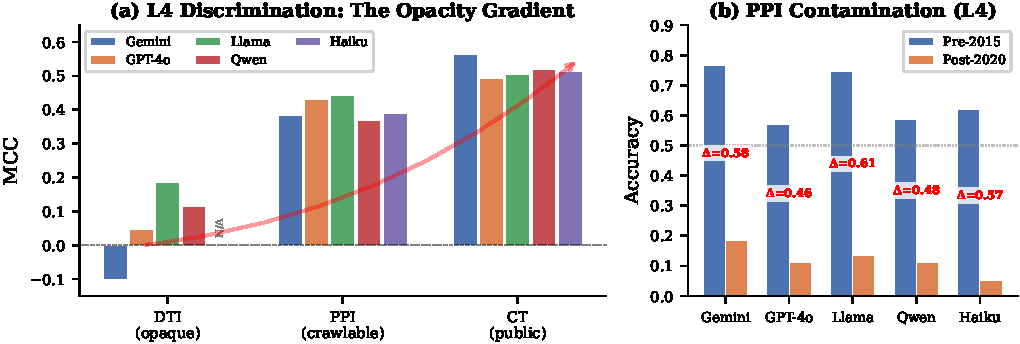
\includegraphics[width=\textwidth]{figures/fig3_l4_gradient.pdf}
\caption{The opacity gradient. \textbf{(a)} L4 discrimination (MCC) across domains for four common models (+Haiku for CT/PPI). Performance increases with data accessibility: DTI (opaque databases) $\to$ PPI (crawlable) $\to$ CT (public). Dashed line: MCC~=~0. \textbf{(b)} PPI contamination: pre-2015 vs.\ post-2020 accuracy. All models show $>$0.35 gaps, confirming memorization. $\Delta$ values in red.}
\label{fig:gradient}
\end{figure}
